\section{実装}
本章では提案システムの実装について述べる。まず3章で述べた設計を実装する際に生じる課題の解決方法について述べた後、システムの動作について述べる。

%現在の提案システムの実装はサーバマシンとクライアントマシンがXMPPサーバから取得した情報をもとに直接リンクを張ってクラウドゲーミング通信を展開する方式になっている。クラウドゲームサーバ/クライアントにはオープンソースクラウドゲーミングプラットフォームであるGamingAnywhereを使用している。また、パブリッククラウド等で展開しているサービスではなく、一般のユーザコンピュータでサービスを展開する手法特有の課題とその対処についても本章で述べる。


%以下ではそれぞれの課題の解決方法を述べる。

\subsection{VCコントローラとエージェントの連携}
VCコントローラと遊休コンピュータ上で動作するVCホストエージェントとの通信の課題についてはgRPC\cite{grpc}を用いる。gRPCはGoogleが開発しているオープンソースのRPCフレームワークで、異なるコンピュータ間情報をやり取りするために使用される。gRPCではクライアントアプリケーションがローカルで実装されたメソッドを使用するかのようにサーバアプリケーションのメソッドを直接呼び出すことができるため、分散アプリケーション等の実装に適している(図\ref{fig:grpc})。サーバ側ではサービスを定義してそのインターフェースを実装する。クライアント側ではサーバと同じメソッドを提供するスタブを介してサーバアプリケーションの機能を使えるようにしているのが特徴である。

gRPCのResponse Streaming gRPCという機能は、単一の要求に対して複数のレスポンスを任意のタイミングで返すことが可能である。これを使用することで、VCクライアントが送信した単一のゲームプレイ要求に対して、ACKや起動報告、実行終了時の完了報告、エラーの通知など様々なレスポンスを返すことができる。

\begin{figure*}[t]
    \centering
    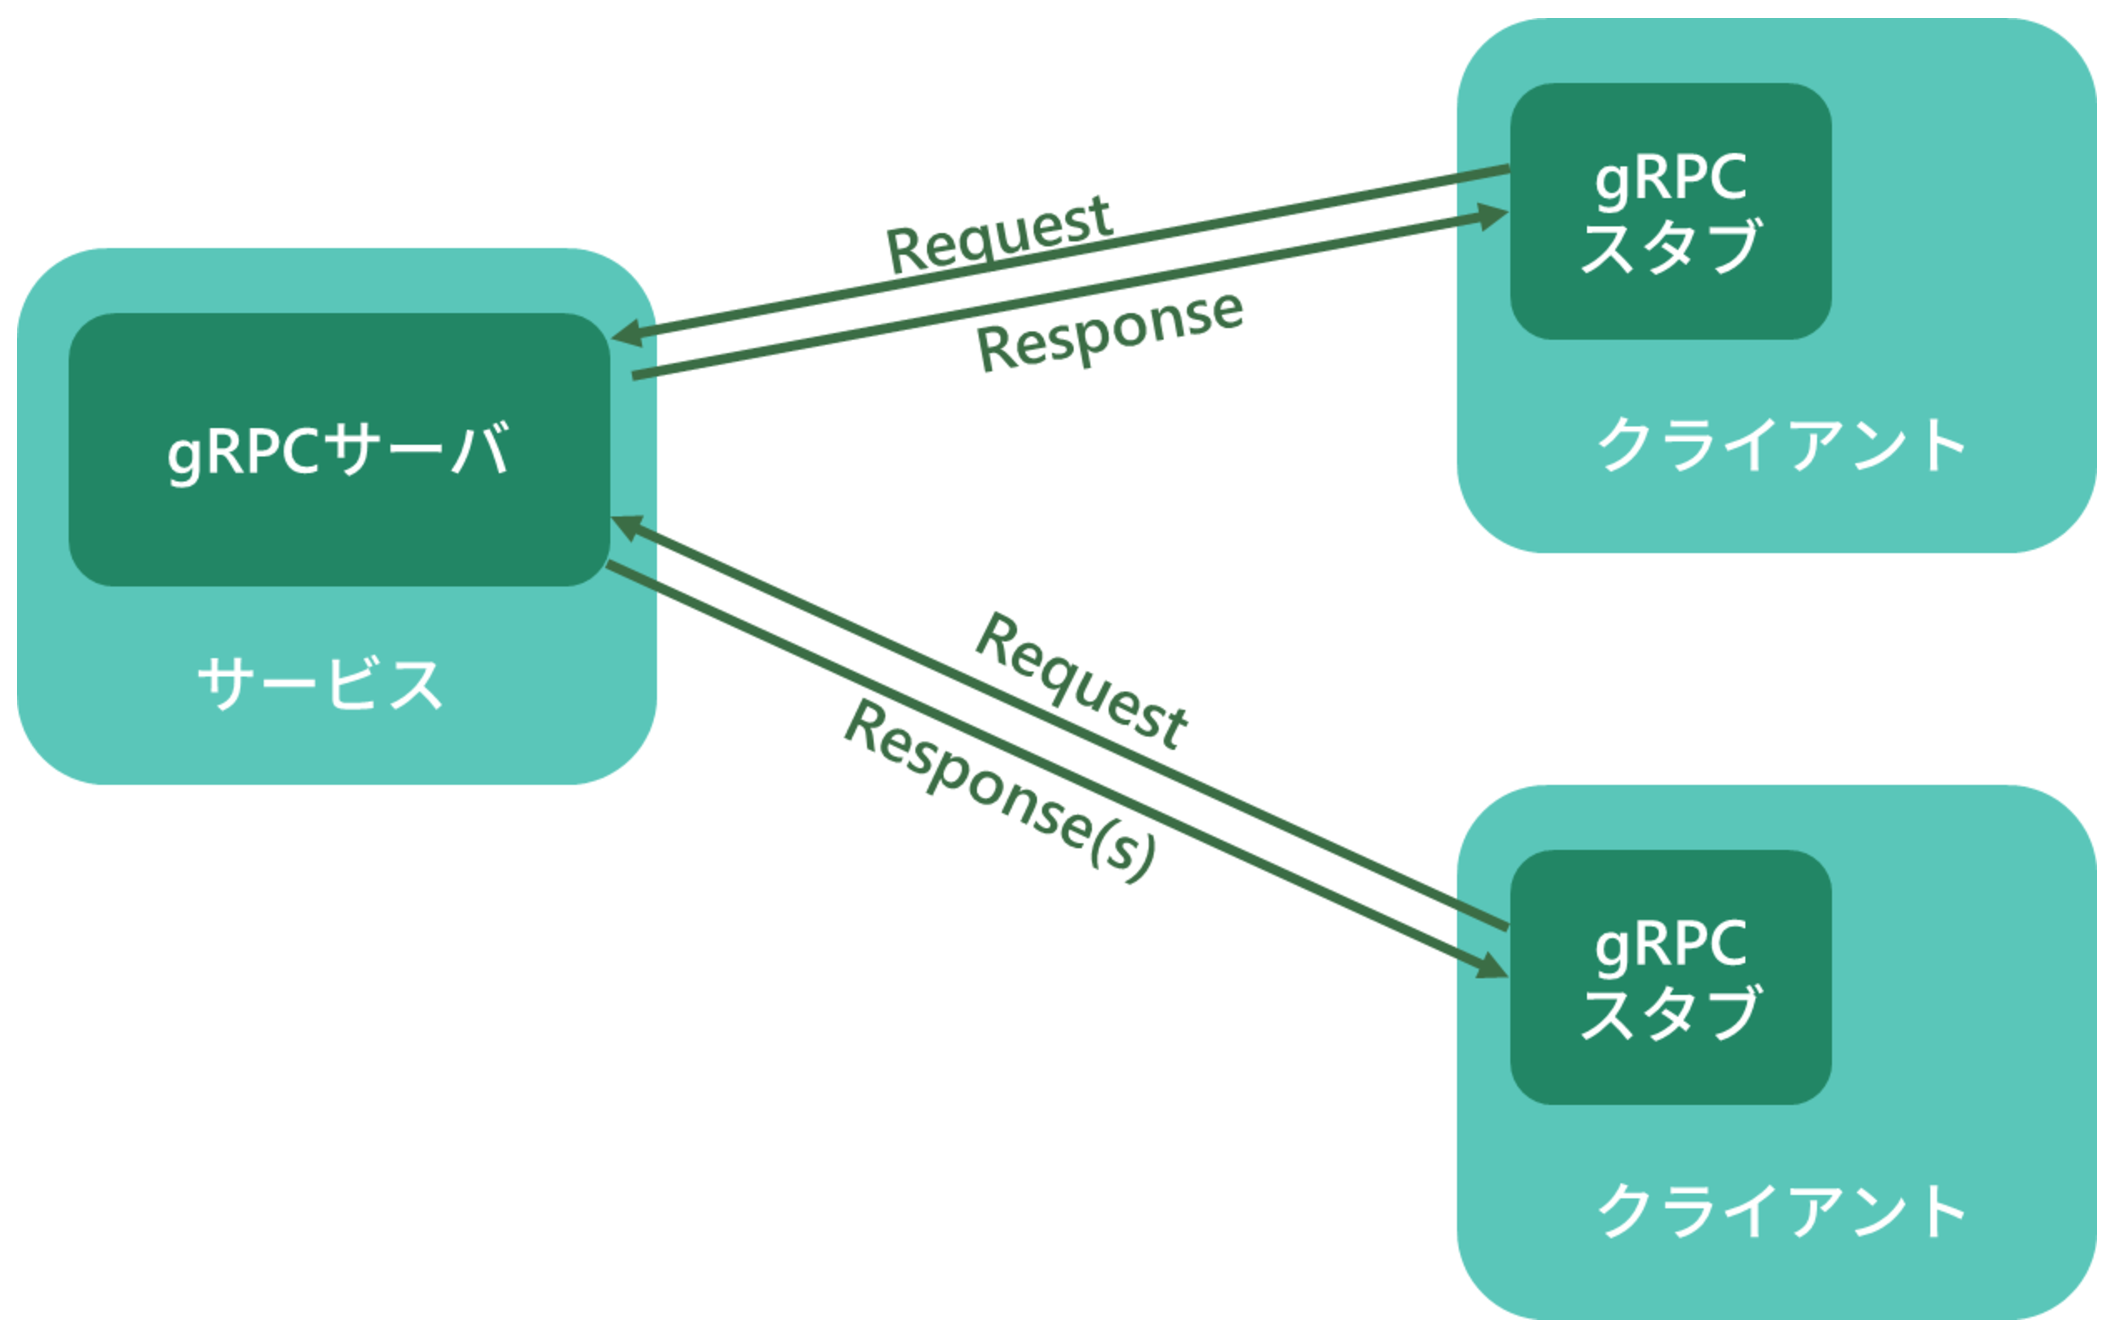
\includegraphics[width=0.8\textwidth,keepaspectratio,clip]{img/grpc.eps}
    \caption{gRPCの概要}
    \label{fig:grpc}
\end{figure*}

\subsection{クラウドゲームサーバ/クライアント間のP2P通信}
実際にリモートでのゲームプレイを実現するクラウドゲームサーバとクラウドゲームクライアントにはGamingAnywhereを使用する。遊休コンピュータ上にGamingAnywhereサーバ、プレイヤーPC上にGamingAnywhereクライアントを起動し、GamingAnywhereサーバが展開するRTSPサーバにクライアントが接続することでクラウドゲームのプレイが開始される。

ここで、ユーザコンピュータで動作するGamingAnywhereサーバ/クライアント間で双方向的な直接通信を行えないという問題がある。この問題の解決策として、遊休コンピュータおよびプレイヤーPCのファイアウォールを解除する、あるいは特定の通信を許可する設定をするという方法がある。しかし、これはセキュリティ上の危険や、煩雑な設定をユーザに強いるという課題がある。

ボランティアコンピューティングをクラウドゲーミングにおいて活用するにあたって、NATやファイアウォールの背後にあるユーザコンピュータのペアを安全かつ透過的に接続することが必要である。また、遊休コンピュータを提供するボランティアやプレイヤーが行う設定は少ないことが好ましい。

そこで、本研究ではGamingAnywhereの通信を行うリンクに対しEdgeVPN\cite{edgevpn}を使用する。
EdgeVPNは、分散コンピューティング環境のエッジに存在するリソース間の通信にスケーラブルなVPNオーバレイを展開するためのオープンソースソフトウェアである。EdgeVPNはIP-over-P2P(IPOP)プロジェクト\cite{ipop}の進化版である。IPOPは、個人の端末を対象としたIPベースのP2Pオーバレイであり、一元化されたユーザー/グループ管理をサポートしている。EdgeVPNを使用することで、エッジデバイス同士が、NAT/ファイアウォール、およびクラウドコンピューティングリソースの背後にあるネットワークアドレスに透過的に接続し、インターネットを介したトラフィックをP2Pで暗号化およびトンネリングすることができる。また、EdgeVPNはXMPPプロトコル\cite{xmpp}を使用してピアとの接続情報を検出および交換する。パケット交換とルーティングは分散されているため、スケーラブルなP2Pオーバレイを展開しつつ、メンバーシップの一元管理も可能である。

EdgeVPNはピア間でカプセル化/暗号化されたイーサネットフレームを伝送する仮想リンクの構築に、Justeら\cite{tincan}が開発したTinCanを使用している。TinCanは、XMPPサーバを使用してエンドツーエンドのVPNトンネルをブートストラップすることにより、コントローラとデータパスを分離するモデルを実現している。また、ノードが接続先に自身のパブリックIPやポートを知らせるためのリフレクションサービスとしてSTUNプロトコル\cite{stun}を使用する。一方、制限の強いファイアウォールやSymmetric NATの背後にあり直接P2P接続を構築できないノードがある場合はリレーサービスとしてTURNプロトコル\cite{turn}を実行するサーバによりトラフィックをプロキシしている。

\subsection{システム動作}
本節ではシステムの動作のシーケンスについて述べる。まず始めにクラウド上に存在するXMPPサーバを使用して、プレイヤーPCと遊休コンピュータがgRPCおよびEdgeVPNのリンクを張るための接続情報をそれぞれに通知する(図\ref{fig:seq}矢印1)。次に、プレイヤーの希望に応じて、プレイヤーPC上のVCクライアントエージェントがgRPCクライアントとして、遊休コンピュータで動作するVCホストエージェント上のgRPCサーバにゲーム起動要求を送信する(矢印2)。これを受信したVCホストエージェントは、クラウドゲームサーバの役割を果たすGamingAnywhereサーバとプレイヤーが指定した所望のゲームを起動し(矢印3)、GamingAnywhereサーバがゲーム画面のキャプチャを開始した後(矢印4)、了解を返す(矢印5)。その後、遊休コンピュータとプレイヤーPC間にEdgeVPNのリンクを張り、プレイヤーPCがGamingAnywhereクライアントを起動して、トンネルを介してGamingAnywhereサーバに接続することでゲームプレイを開始する(矢印6)。また、ゲームプレイ終了時はGamingAnywhereクライアントの終了によって接続の切断がGamingAnywhereサーバに通知されるため、それを観測することでVCクライアントエージェントは終了を検知し、GamingAnywhereとゲームを終了する(矢印7)。

\begin{figure*}[t]
    \centering
    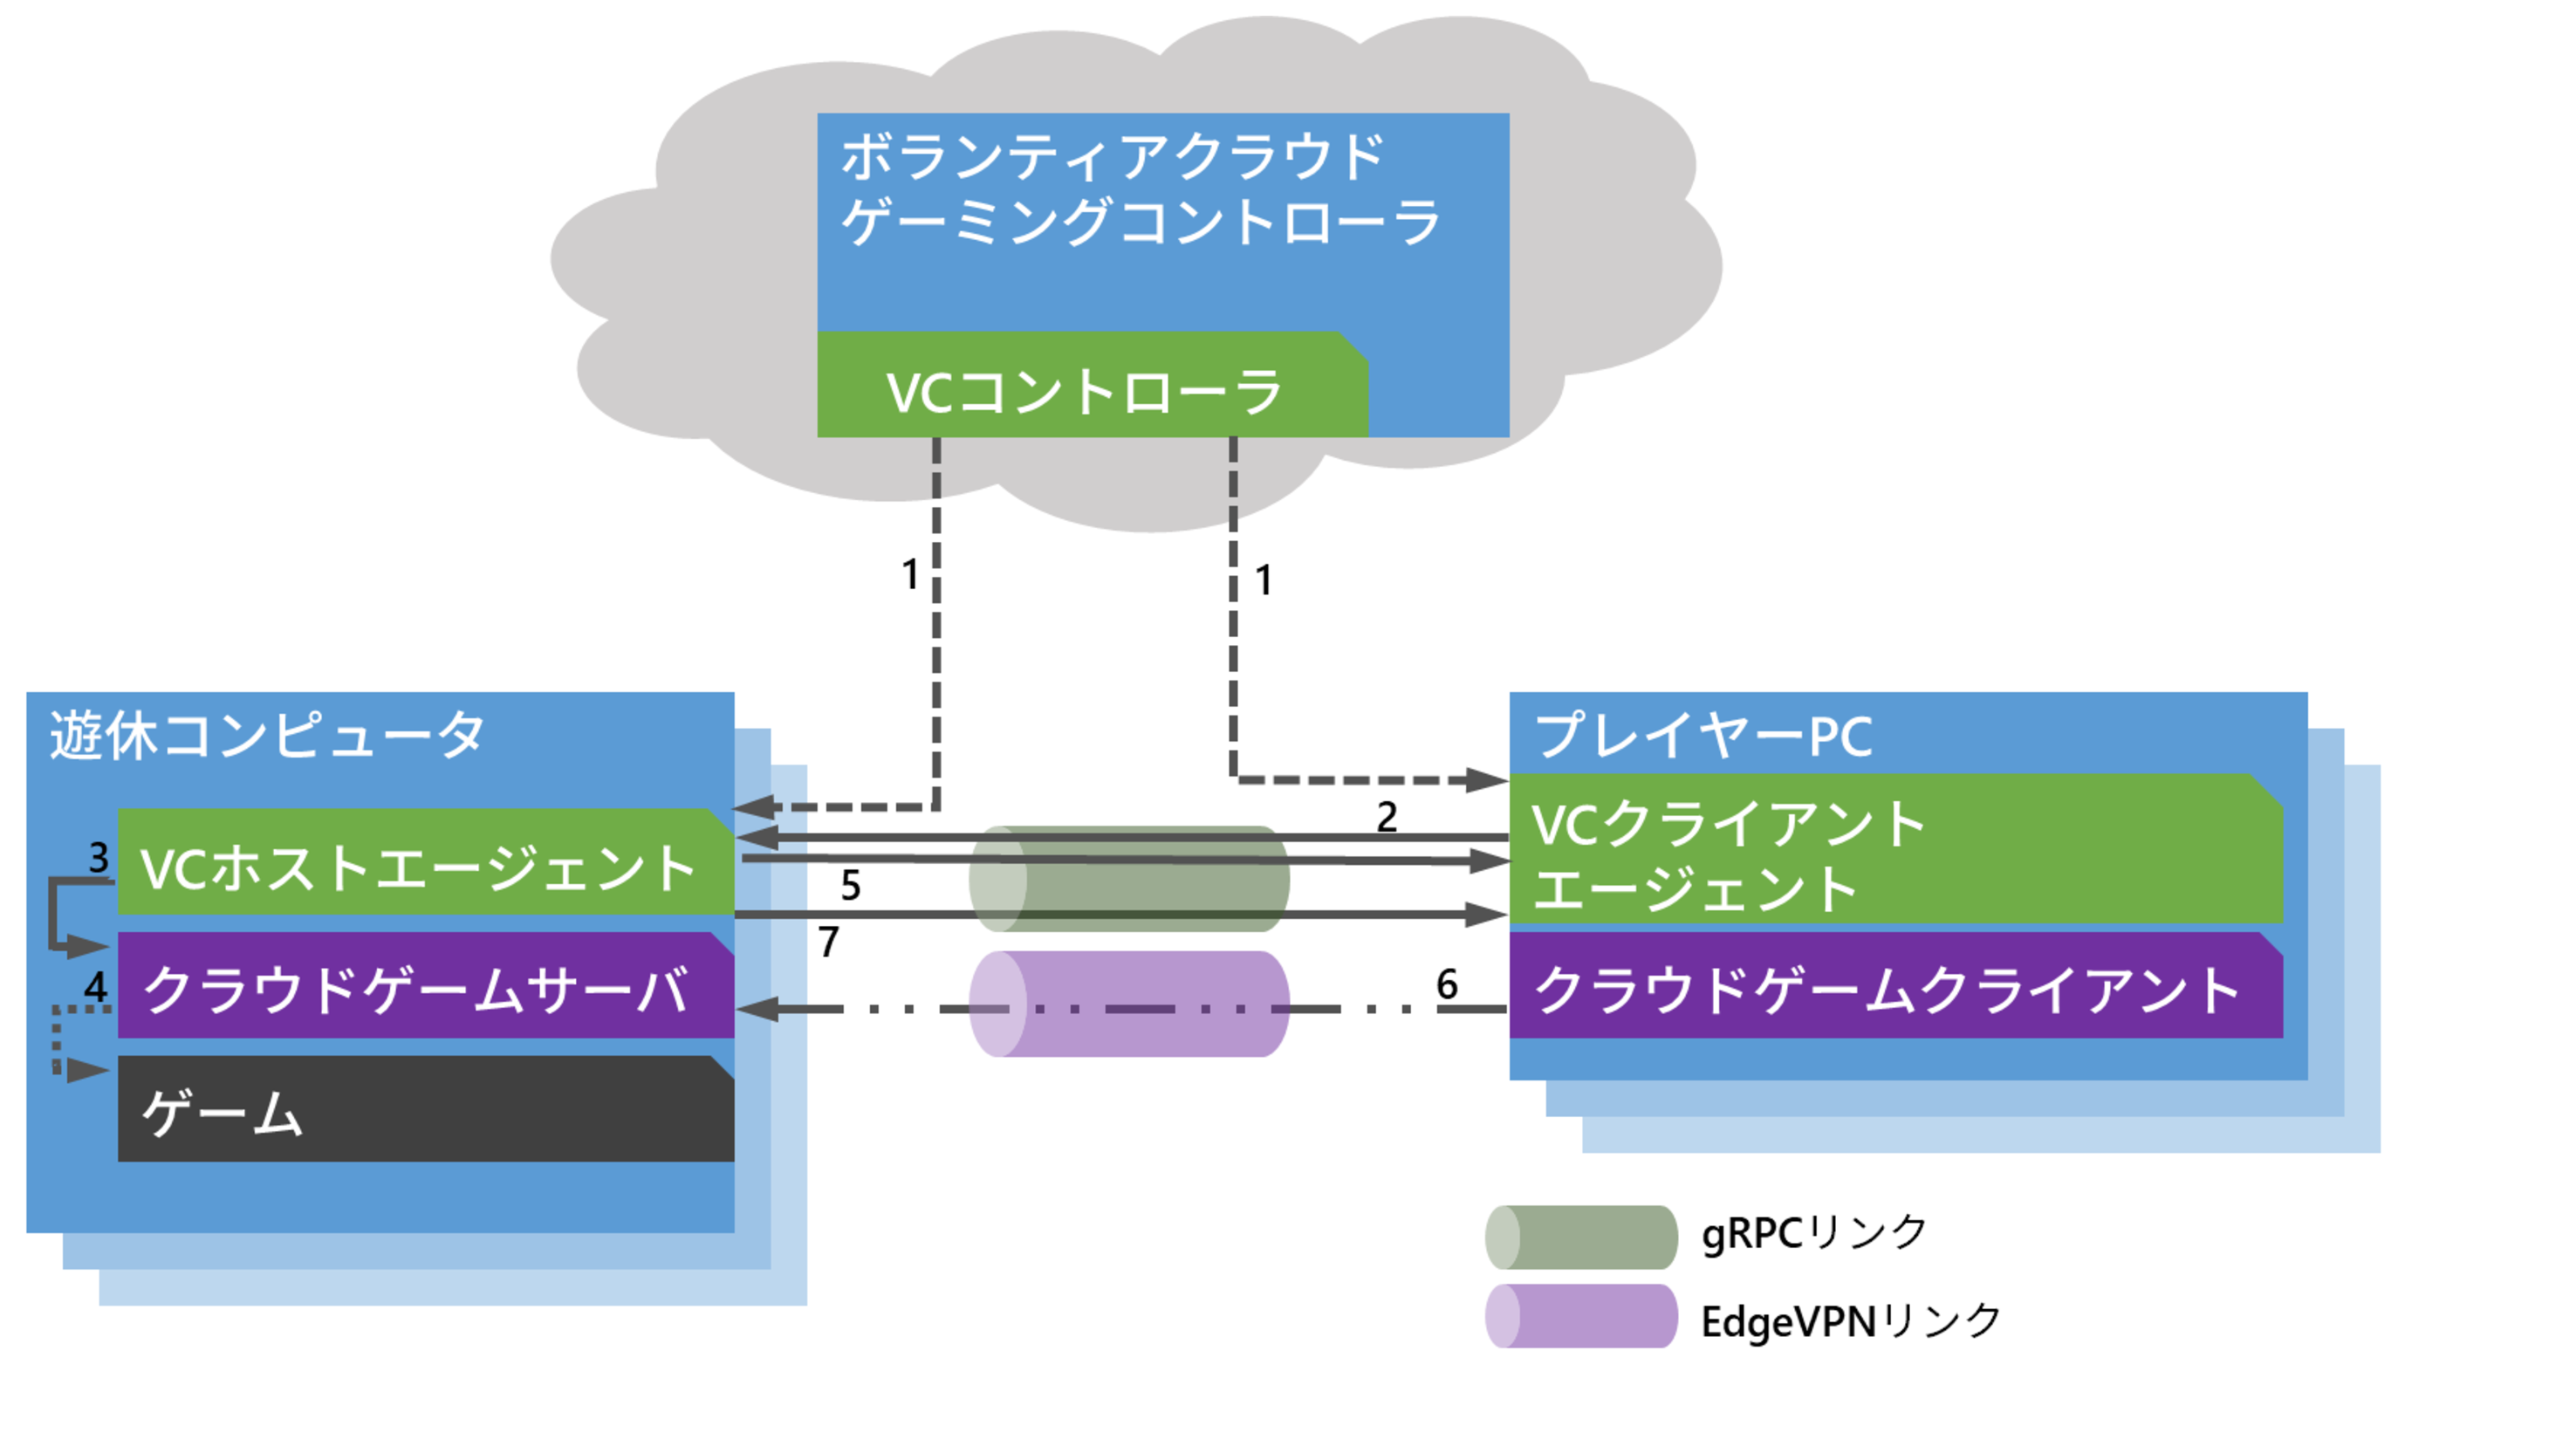
\includegraphics[width=0.8\textwidth,keepaspectratio,clip]{img/sequence.eps}
    \caption{システム動作}
    \label{fig:seq}
\end{figure*}

